\documentclass[twoside]{book}

% Packages required by doxygen
\usepackage{fixltx2e}
\usepackage{calc}
\usepackage{doxygen}
\usepackage[export]{adjustbox} % also loads graphicx
\usepackage{graphicx}
\usepackage[utf8]{inputenc}
\usepackage{makeidx}
\usepackage{multicol}
\usepackage{multirow}
\PassOptionsToPackage{warn}{textcomp}
\usepackage{textcomp}
\usepackage[nointegrals]{wasysym}
\usepackage[table]{xcolor}

% Font selection
\usepackage[T1]{fontenc}
\usepackage[scaled=.90]{helvet}
\usepackage{courier}
\usepackage{amssymb}
\usepackage{sectsty}
\renewcommand{\familydefault}{\sfdefault}
\allsectionsfont{%
  \fontseries{bc}\selectfont%
  \color{darkgray}%
}
\renewcommand{\DoxyLabelFont}{%
  \fontseries{bc}\selectfont%
  \color{darkgray}%
}
\newcommand{\+}{\discretionary{\mbox{\scriptsize$\hookleftarrow$}}{}{}}

% Page & text layout
\usepackage{geometry}
\geometry{%
  a4paper,%
  top=2.5cm,%
  bottom=2.5cm,%
  left=2.5cm,%
  right=2.5cm%
}
\tolerance=750
\hfuzz=15pt
\hbadness=750
\setlength{\emergencystretch}{15pt}
\setlength{\parindent}{0cm}
\setlength{\parskip}{3ex plus 2ex minus 2ex}
\makeatletter
\renewcommand{\paragraph}{%
  \@startsection{paragraph}{4}{0ex}{-1.0ex}{1.0ex}{%
    \normalfont\normalsize\bfseries\SS@parafont%
  }%
}
\renewcommand{\subparagraph}{%
  \@startsection{subparagraph}{5}{0ex}{-1.0ex}{1.0ex}{%
    \normalfont\normalsize\bfseries\SS@subparafont%
  }%
}
\makeatother

% Headers & footers
\usepackage{fancyhdr}
\pagestyle{fancyplain}
\fancyhead[LE]{\fancyplain{}{\bfseries\thepage}}
\fancyhead[CE]{\fancyplain{}{}}
\fancyhead[RE]{\fancyplain{}{\bfseries\leftmark}}
\fancyhead[LO]{\fancyplain{}{\bfseries\rightmark}}
\fancyhead[CO]{\fancyplain{}{}}
\fancyhead[RO]{\fancyplain{}{\bfseries\thepage}}
\fancyfoot[LE]{\fancyplain{}{}}
\fancyfoot[CE]{\fancyplain{}{}}
\fancyfoot[RE]{\fancyplain{}{\bfseries\scriptsize Generated by Doxygen }}
\fancyfoot[LO]{\fancyplain{}{\bfseries\scriptsize Generated by Doxygen }}
\fancyfoot[CO]{\fancyplain{}{}}
\fancyfoot[RO]{\fancyplain{}{}}
\renewcommand{\footrulewidth}{0.4pt}
\renewcommand{\chaptermark}[1]{%
  \markboth{#1}{}%
}
\renewcommand{\sectionmark}[1]{%
  \markright{\thesection\ #1}%
}

% Indices & bibliography
\usepackage{natbib}
\usepackage[titles]{tocloft}
\setcounter{tocdepth}{3}
\setcounter{secnumdepth}{5}
\makeindex

% Hyperlinks (required, but should be loaded last)
\usepackage{ifpdf}
\ifpdf
  \usepackage[pdftex,pagebackref=true]{hyperref}
\else
  \usepackage[ps2pdf,pagebackref=true]{hyperref}
\fi
\hypersetup{%
  colorlinks=true,%
  linkcolor=blue,%
  citecolor=blue,%
  unicode%
}

% Custom commands
\newcommand{\clearemptydoublepage}{%
  \newpage{\pagestyle{empty}\cleardoublepage}%
}

\usepackage{caption}
\captionsetup{labelsep=space,justification=centering,font={bf},singlelinecheck=off,skip=4pt,position=top}

%===== C O N T E N T S =====

\begin{document}

% Titlepage & ToC
\hypersetup{pageanchor=false,
             bookmarksnumbered=true,
             pdfencoding=unicode
            }
\pagenumbering{roman}
\begin{titlepage}
\vspace*{7cm}
\begin{center}%
{\Large Anti-\/\+Aliasing }\\
\vspace*{1cm}
{\large Generated by Doxygen 1.8.11}\\
\end{center}
\end{titlepage}
\clearemptydoublepage
\tableofcontents
\clearemptydoublepage
\pagenumbering{arabic}
\hypersetup{pageanchor=true}

%--- Begin generated contents ---
\chapter{Hierarchical Index}
\section{Class Hierarchy}
This inheritance list is sorted roughly, but not completely, alphabetically\+:\begin{DoxyCompactList}
\item \contentsline{section}{Canvas}{\pageref{classCanvas}}{}
\item \contentsline{section}{Draw}{\pageref{classDraw}}{}
\begin{DoxyCompactList}
\item \contentsline{section}{Draw\+Sampling}{\pageref{classDrawSampling}}{}
\begin{DoxyCompactList}
\item \contentsline{section}{Draw\+Kernel}{\pageref{classDrawKernel}}{}
\end{DoxyCompactList}
\item \contentsline{section}{Draw\+Width}{\pageref{classDrawWidth}}{}
\end{DoxyCompactList}
\end{DoxyCompactList}

\chapter{Class Index}
\section{Class List}
Here are the classes, structs, unions and interfaces with brief descriptions\+:\begin{DoxyCompactList}
\item\contentsline{section}{\hyperlink{classCanvas}{Canvas} \\*Interface to Open\+CV }{\pageref{classCanvas}}{}
\item\contentsline{section}{\hyperlink{classDraw}{Draw} \\*Plain draw-\/line algorithm }{\pageref{classDraw}}{}
\item\contentsline{section}{\hyperlink{classDrawKernel}{Draw\+Kernel} \\*Kernel algorithm, i.\+e }{\pageref{classDrawKernel}}{}
\item\contentsline{section}{\hyperlink{classDrawSampling}{Draw\+Sampling} \\*Uniform sampling algorithm }{\pageref{classDrawSampling}}{}
\item\contentsline{section}{\hyperlink{classDrawWidth}{Draw\+Width} \\*\hyperlink{classDraw}{Draw} lines with a width }{\pageref{classDrawWidth}}{}
\end{DoxyCompactList}

\chapter{File Index}
\section{File List}
Here is a list of all files with brief descriptions\+:\begin{DoxyCompactList}
\item\contentsline{section}{\hyperlink{canvas_8h}{canvas.\+h} }{\pageref{canvas_8h}}{}
\item\contentsline{section}{\hyperlink{const_8h}{const.\+h} }{\pageref{const_8h}}{}
\item\contentsline{section}{\hyperlink{draw_8cpp}{draw.\+cpp} }{\pageref{draw_8cpp}}{}
\item\contentsline{section}{\hyperlink{draw_8h}{draw.\+h} }{\pageref{draw_8h}}{}
\item\contentsline{section}{\hyperlink{drawkernel_8h}{drawkernel.\+h} }{\pageref{drawkernel_8h}}{}
\item\contentsline{section}{\hyperlink{drawsampling_8cpp}{drawsampling.\+cpp} }{\pageref{drawsampling_8cpp}}{}
\item\contentsline{section}{\hyperlink{drawsampling_8h}{drawsampling.\+h} }{\pageref{drawsampling_8h}}{}
\item\contentsline{section}{\hyperlink{drawwidth_8cpp}{drawwidth.\+cpp} }{\pageref{drawwidth_8cpp}}{}
\item\contentsline{section}{\hyperlink{drawwidth_8h}{drawwidth.\+h} }{\pageref{drawwidth_8h}}{}
\item\contentsline{section}{\hyperlink{main_8cpp}{main.\+cpp} }{\pageref{main_8cpp}}{}
\end{DoxyCompactList}

\chapter{Class Documentation}
\hypertarget{classCanvas}{}\section{Canvas Class Reference}
\label{classCanvas}\index{Canvas@{Canvas}}


Interface to Open\+CV.  




{\ttfamily \#include $<$canvas.\+h$>$}



Collaboration diagram for Canvas\+:
\nopagebreak
\begin{figure}[H]
\begin{center}
\leavevmode
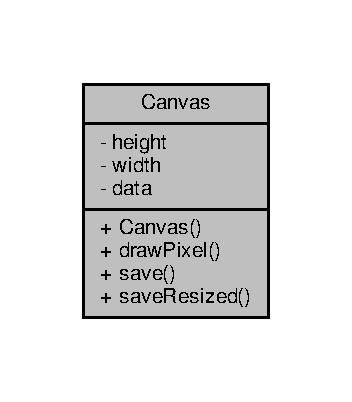
\includegraphics[width=169pt]{classCanvas__coll__graph}
\end{center}
\end{figure}
\subsection*{Public Member Functions}
\begin{DoxyCompactItemize}
\item 
\hyperlink{classCanvas_a04e5495c637170cd93c20dbcc56b7cce}{Canvas} (int \+\_\+height, int \+\_\+width, const \hyperlink{canvas_8h_a084a39206618848fb8bc9187d3758c87}{Color} \&background)
\begin{DoxyCompactList}\small\item\em In H\+SV color space. \end{DoxyCompactList}\item 
void \hyperlink{classCanvas_a74e163f47b09d23afc273c5024918280}{draw\+Pixel} (int x, int y, const \hyperlink{canvas_8h_a084a39206618848fb8bc9187d3758c87}{Color} \&color, int alphaU, int alphaD)
\begin{DoxyCompactList}\small\item\em \hyperlink{classDraw}{Draw} a pixel with given transparency alpha = alphaU / alphaD. \end{DoxyCompactList}\item 
void \hyperlink{classCanvas_a2fcf1999f81d5cbbb55271b7f3db1565}{save} (const char $\ast$filename) const 
\begin{DoxyCompactList}\small\item\em Save to file. \end{DoxyCompactList}\item 
void \hyperlink{classCanvas_a2d3e01d8ec83c99e36b76f780c1bfa3e}{save\+Resized} (const char $\ast$filename, int \+\_\+height, int \+\_\+width) const 
\end{DoxyCompactItemize}
\subsection*{Private Attributes}
\begin{DoxyCompactItemize}
\item 
int \hyperlink{classCanvas_aada7c1a775b50c422801d477e82a53ec}{height}
\item 
int \hyperlink{classCanvas_a31434dcd520abfa1c1f3fb778514d173}{width}
\item 
cv\+::\+Mat3b \hyperlink{classCanvas_ac5e24c180dd682c1fe9f57f4f11d5db6}{data}
\end{DoxyCompactItemize}


\subsection{Detailed Description}
Interface to Open\+CV. 

\subsection{Constructor \& Destructor Documentation}
\index{Canvas@{Canvas}!Canvas@{Canvas}}
\index{Canvas@{Canvas}!Canvas@{Canvas}}
\subsubsection[{\texorpdfstring{Canvas(int \+\_\+height, int \+\_\+width, const Color \&background)}{Canvas(int _height, int _width, const Color &background)}}]{\setlength{\rightskip}{0pt plus 5cm}Canvas\+::\+Canvas (
\begin{DoxyParamCaption}
\item[{int}]{\+\_\+height, }
\item[{int}]{\+\_\+width, }
\item[{const {\bf Color} \&}]{background}
\end{DoxyParamCaption}
)\hspace{0.3cm}{\ttfamily [inline]}}\hypertarget{classCanvas_a04e5495c637170cd93c20dbcc56b7cce}{}\label{classCanvas_a04e5495c637170cd93c20dbcc56b7cce}


In H\+SV color space. 

Initialize an empty image 

\subsection{Member Function Documentation}
\index{Canvas@{Canvas}!draw\+Pixel@{draw\+Pixel}}
\index{draw\+Pixel@{draw\+Pixel}!Canvas@{Canvas}}
\subsubsection[{\texorpdfstring{draw\+Pixel(int x, int y, const Color \&color, int alpha\+U, int alpha\+D)}{drawPixel(int x, int y, const Color &color, int alphaU, int alphaD)}}]{\setlength{\rightskip}{0pt plus 5cm}void Canvas\+::draw\+Pixel (
\begin{DoxyParamCaption}
\item[{int}]{x, }
\item[{int}]{y, }
\item[{const {\bf Color} \&}]{color, }
\item[{int}]{alphaU, }
\item[{int}]{alphaD}
\end{DoxyParamCaption}
)\hspace{0.3cm}{\ttfamily [inline]}}\hypertarget{classCanvas_a74e163f47b09d23afc273c5024918280}{}\label{classCanvas_a74e163f47b09d23afc273c5024918280}


\hyperlink{classDraw}{Draw} a pixel with given transparency alpha = alphaU / alphaD. 

\index{Canvas@{Canvas}!save@{save}}
\index{save@{save}!Canvas@{Canvas}}
\subsubsection[{\texorpdfstring{save(const char $\ast$filename) const }{save(const char *filename) const }}]{\setlength{\rightskip}{0pt plus 5cm}void Canvas\+::save (
\begin{DoxyParamCaption}
\item[{const char $\ast$}]{filename}
\end{DoxyParamCaption}
) const\hspace{0.3cm}{\ttfamily [inline]}}\hypertarget{classCanvas_a2fcf1999f81d5cbbb55271b7f3db1565}{}\label{classCanvas_a2fcf1999f81d5cbbb55271b7f3db1565}


Save to file. 

\index{Canvas@{Canvas}!save\+Resized@{save\+Resized}}
\index{save\+Resized@{save\+Resized}!Canvas@{Canvas}}
\subsubsection[{\texorpdfstring{save\+Resized(const char $\ast$filename, int \+\_\+height, int \+\_\+width) const }{saveResized(const char *filename, int _height, int _width) const }}]{\setlength{\rightskip}{0pt plus 5cm}void Canvas\+::save\+Resized (
\begin{DoxyParamCaption}
\item[{const char $\ast$}]{filename, }
\item[{int}]{\+\_\+height, }
\item[{int}]{\+\_\+width}
\end{DoxyParamCaption}
) const\hspace{0.3cm}{\ttfamily [inline]}}\hypertarget{classCanvas_a2d3e01d8ec83c99e36b76f780c1bfa3e}{}\label{classCanvas_a2d3e01d8ec83c99e36b76f780c1bfa3e}


\subsection{Member Data Documentation}
\index{Canvas@{Canvas}!data@{data}}
\index{data@{data}!Canvas@{Canvas}}
\subsubsection[{\texorpdfstring{data}{data}}]{\setlength{\rightskip}{0pt plus 5cm}cv\+::\+Mat3b Canvas\+::data\hspace{0.3cm}{\ttfamily [private]}}\hypertarget{classCanvas_ac5e24c180dd682c1fe9f57f4f11d5db6}{}\label{classCanvas_ac5e24c180dd682c1fe9f57f4f11d5db6}
\index{Canvas@{Canvas}!height@{height}}
\index{height@{height}!Canvas@{Canvas}}
\subsubsection[{\texorpdfstring{height}{height}}]{\setlength{\rightskip}{0pt plus 5cm}int Canvas\+::height\hspace{0.3cm}{\ttfamily [private]}}\hypertarget{classCanvas_aada7c1a775b50c422801d477e82a53ec}{}\label{classCanvas_aada7c1a775b50c422801d477e82a53ec}
\index{Canvas@{Canvas}!width@{width}}
\index{width@{width}!Canvas@{Canvas}}
\subsubsection[{\texorpdfstring{width}{width}}]{\setlength{\rightskip}{0pt plus 5cm}int Canvas\+::width\hspace{0.3cm}{\ttfamily [private]}}\hypertarget{classCanvas_a31434dcd520abfa1c1f3fb778514d173}{}\label{classCanvas_a31434dcd520abfa1c1f3fb778514d173}


The documentation for this class was generated from the following file\+:\begin{DoxyCompactItemize}
\item 
\hyperlink{canvas_8h}{canvas.\+h}\end{DoxyCompactItemize}

\hypertarget{classDraw}{}\section{Draw Class Reference}
\label{classDraw}\index{Draw@{Draw}}


Plain draw-\/line algorithm.  




{\ttfamily \#include $<$draw.\+h$>$}



Inheritance diagram for Draw\+:\nopagebreak
\begin{figure}[H]
\begin{center}
\leavevmode
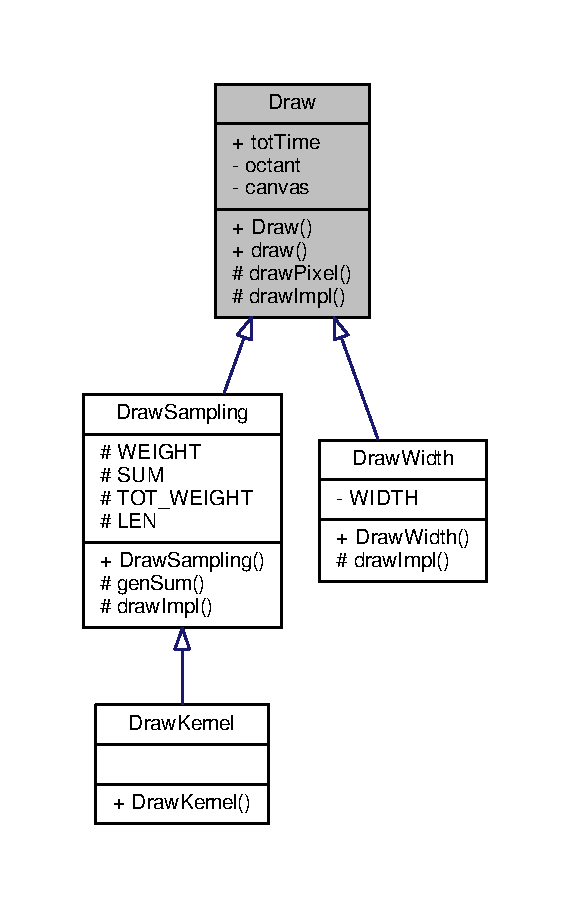
\includegraphics[width=274pt]{classDraw__inherit__graph}
\end{center}
\end{figure}


Collaboration diagram for Draw\+:\nopagebreak
\begin{figure}[H]
\begin{center}
\leavevmode
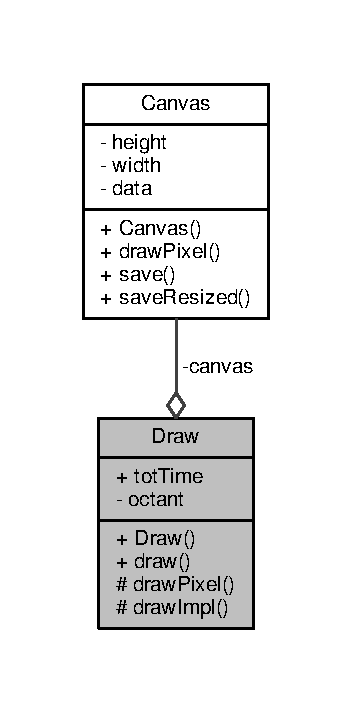
\includegraphics[width=169pt]{classDraw__coll__graph}
\end{center}
\end{figure}
\subsection*{Public Member Functions}
\begin{DoxyCompactItemize}
\item 
\hyperlink{classDraw_ab01ae8a362d3c42015e7c1634109fc7b}{Draw} (\hyperlink{classCanvas}{Canvas} \&\+\_\+canvas)
\item 
void \hyperlink{classDraw_a4948f44fd8928e53243deb5348567bb0}{draw} (int x0, int y0, int x1, int y1, const \hyperlink{canvas_8h_a084a39206618848fb8bc9187d3758c87}{Color} \&color)
\begin{DoxyCompactList}\small\item\em \hyperlink{classDraw}{Draw} a line\+: (x0, y0) -\/$>$ (x1, y1) \end{DoxyCompactList}\end{DoxyCompactItemize}
\subsection*{Public Attributes}
\begin{DoxyCompactItemize}
\item 
double \hyperlink{classDraw_aca821acc8a6745c5ef690ab84f65be7f}{tot\+Time}
\end{DoxyCompactItemize}
\subsection*{Protected Member Functions}
\begin{DoxyCompactItemize}
\item 
void \hyperlink{classDraw_afabd95d3a324312417127a468710fd8a}{draw\+Pixel} (int x, int y, const \hyperlink{canvas_8h_a084a39206618848fb8bc9187d3758c87}{Color} \&color, int alphaU=1, int alphaD=1)
\begin{DoxyCompactList}\small\item\em \hyperlink{classDraw}{Draw} a pixel accroding to current octant alpha = alphaU / alphaD. \end{DoxyCompactList}\item 
virtual void \hyperlink{classDraw_ac9f2fe7c73db00834df73437767fa3ce}{draw\+Impl} (int x0, int y0, int x1, int y1, const \hyperlink{canvas_8h_a084a39206618848fb8bc9187d3758c87}{Color} \&color)
\begin{DoxyCompactList}\small\item\em Implementation. \end{DoxyCompactList}\end{DoxyCompactItemize}
\subsection*{Private Attributes}
\begin{DoxyCompactItemize}
\item 
int \hyperlink{classDraw_a9a0e070ec76f4f9c95fa7e717c34bdbc}{octant}
\begin{DoxyCompactList}\small\item\em Octant in \mbox{[}0, 4) \textbackslash{}2$\vert$1/ \subsubsection*{3/0 }\end{DoxyCompactList}\item 
\hyperlink{classCanvas}{Canvas} \& \hyperlink{classDraw_a72ed77716d9eb7068414f0e4e00753bd}{canvas}
\end{DoxyCompactItemize}


\subsection{Detailed Description}
Plain draw-\/line algorithm. 

\subsection{Constructor \& Destructor Documentation}
\index{Draw@{Draw}!Draw@{Draw}}
\index{Draw@{Draw}!Draw@{Draw}}
\subsubsection[{\texorpdfstring{Draw(\+Canvas \&\+\_\+canvas)}{Draw(Canvas &_canvas)}}]{\setlength{\rightskip}{0pt plus 5cm}Draw\+::\+Draw (
\begin{DoxyParamCaption}
\item[{{\bf Canvas} \&}]{\+\_\+canvas}
\end{DoxyParamCaption}
)\hspace{0.3cm}{\ttfamily [inline]}}\hypertarget{classDraw_ab01ae8a362d3c42015e7c1634109fc7b}{}\label{classDraw_ab01ae8a362d3c42015e7c1634109fc7b}


\subsection{Member Function Documentation}
\index{Draw@{Draw}!draw@{draw}}
\index{draw@{draw}!Draw@{Draw}}
\subsubsection[{\texorpdfstring{draw(int x0, int y0, int x1, int y1, const Color \&color)}{draw(int x0, int y0, int x1, int y1, const Color &color)}}]{\setlength{\rightskip}{0pt plus 5cm}void Draw\+::draw (
\begin{DoxyParamCaption}
\item[{int}]{x0, }
\item[{int}]{y0, }
\item[{int}]{x1, }
\item[{int}]{y1, }
\item[{const {\bf Color} \&}]{color}
\end{DoxyParamCaption}
)}\hypertarget{classDraw_a4948f44fd8928e53243deb5348567bb0}{}\label{classDraw_a4948f44fd8928e53243deb5348567bb0}


\hyperlink{classDraw}{Draw} a line\+: (x0, y0) -\/$>$ (x1, y1) 

\index{Draw@{Draw}!draw\+Impl@{draw\+Impl}}
\index{draw\+Impl@{draw\+Impl}!Draw@{Draw}}
\subsubsection[{\texorpdfstring{draw\+Impl(int x0, int y0, int x1, int y1, const Color \&color)}{drawImpl(int x0, int y0, int x1, int y1, const Color &color)}}]{\setlength{\rightskip}{0pt plus 5cm}void Draw\+::draw\+Impl (
\begin{DoxyParamCaption}
\item[{int}]{x0, }
\item[{int}]{y0, }
\item[{int}]{x1, }
\item[{int}]{y1, }
\item[{const {\bf Color} \&}]{color}
\end{DoxyParamCaption}
)\hspace{0.3cm}{\ttfamily [protected]}, {\ttfamily [virtual]}}\hypertarget{classDraw_ac9f2fe7c73db00834df73437767fa3ce}{}\label{classDraw_ac9f2fe7c73db00834df73437767fa3ce}


Implementation. 

Suppose 0 $<$= slope $<$= 1 

Reimplemented in \hyperlink{classDrawSampling_a3d67fd8278cf17d4cb35958aa1a21e31}{Draw\+Sampling}, and \hyperlink{classDrawWidth_a566f96378bc924c2362551c062612131}{Draw\+Width}.

\index{Draw@{Draw}!draw\+Pixel@{draw\+Pixel}}
\index{draw\+Pixel@{draw\+Pixel}!Draw@{Draw}}
\subsubsection[{\texorpdfstring{draw\+Pixel(int x, int y, const Color \&color, int alpha\+U=1, int alpha\+D=1)}{drawPixel(int x, int y, const Color &color, int alphaU=1, int alphaD=1)}}]{\setlength{\rightskip}{0pt plus 5cm}void Draw\+::draw\+Pixel (
\begin{DoxyParamCaption}
\item[{int}]{x, }
\item[{int}]{y, }
\item[{const {\bf Color} \&}]{color, }
\item[{int}]{alphaU = {\ttfamily 1}, }
\item[{int}]{alphaD = {\ttfamily 1}}
\end{DoxyParamCaption}
)\hspace{0.3cm}{\ttfamily [protected]}}\hypertarget{classDraw_afabd95d3a324312417127a468710fd8a}{}\label{classDraw_afabd95d3a324312417127a468710fd8a}


\hyperlink{classDraw}{Draw} a pixel accroding to current octant alpha = alphaU / alphaD. 



\subsection{Member Data Documentation}
\index{Draw@{Draw}!canvas@{canvas}}
\index{canvas@{canvas}!Draw@{Draw}}
\subsubsection[{\texorpdfstring{canvas}{canvas}}]{\setlength{\rightskip}{0pt plus 5cm}{\bf Canvas}\& Draw\+::canvas\hspace{0.3cm}{\ttfamily [private]}}\hypertarget{classDraw_a72ed77716d9eb7068414f0e4e00753bd}{}\label{classDraw_a72ed77716d9eb7068414f0e4e00753bd}
\index{Draw@{Draw}!octant@{octant}}
\index{octant@{octant}!Draw@{Draw}}
\subsubsection[{\texorpdfstring{octant}{octant}}]{\setlength{\rightskip}{0pt plus 5cm}int Draw\+::octant\hspace{0.3cm}{\ttfamily [private]}}\hypertarget{classDraw_a9a0e070ec76f4f9c95fa7e717c34bdbc}{}\label{classDraw_a9a0e070ec76f4f9c95fa7e717c34bdbc}


Octant in \mbox{[}0, 4) \textbackslash{}2$\vert$1/ \subsubsection*{3/0 }

\index{Draw@{Draw}!tot\+Time@{tot\+Time}}
\index{tot\+Time@{tot\+Time}!Draw@{Draw}}
\subsubsection[{\texorpdfstring{tot\+Time}{totTime}}]{\setlength{\rightskip}{0pt plus 5cm}double Draw\+::tot\+Time}\hypertarget{classDraw_aca821acc8a6745c5ef690ab84f65be7f}{}\label{classDraw_aca821acc8a6745c5ef690ab84f65be7f}


The documentation for this class was generated from the following files\+:\begin{DoxyCompactItemize}
\item 
\hyperlink{draw_8h}{draw.\+h}\item 
\hyperlink{draw_8cpp}{draw.\+cpp}\end{DoxyCompactItemize}

\hypertarget{classDrawKernel}{}\section{Draw\+Kernel Class Reference}
\label{classDrawKernel}\index{Draw\+Kernel@{Draw\+Kernel}}


Kernel algorithm, i.\+e.  




{\ttfamily \#include $<$drawkernel.\+h$>$}



Inheritance diagram for Draw\+Kernel\+:
\nopagebreak
\begin{figure}[H]
\begin{center}
\leavevmode
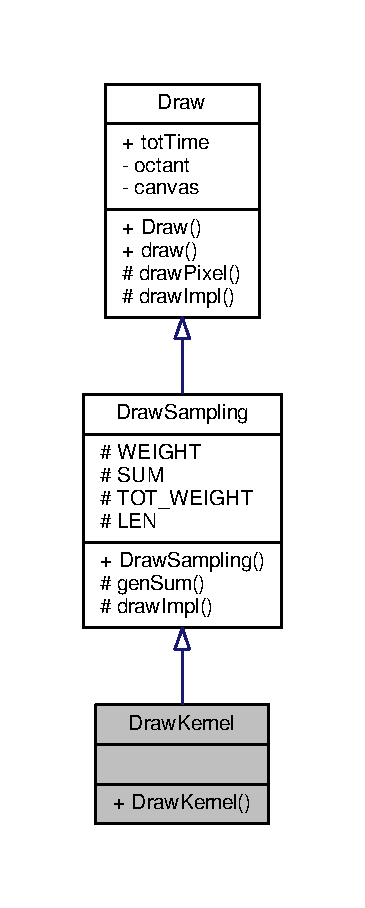
\includegraphics[width=175pt]{classDrawKernel__inherit__graph}
\end{center}
\end{figure}


Collaboration diagram for Draw\+Kernel\+:
\nopagebreak
\begin{figure}[H]
\begin{center}
\leavevmode
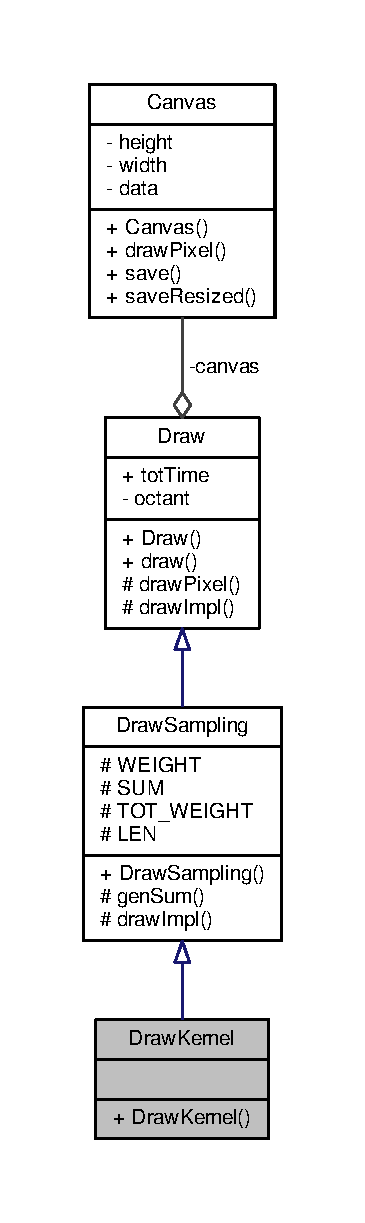
\includegraphics[height=550pt]{classDrawKernel__coll__graph}
\end{center}
\end{figure}
\subsection*{Public Member Functions}
\begin{DoxyCompactItemize}
\item 
\hyperlink{classDrawKernel_a5f419bac95daf351c15a12517df229a6}{Draw\+Kernel} (\hyperlink{classCanvas}{Canvas} \&\hyperlink{classDraw_a72ed77716d9eb7068414f0e4e00753bd}{canvas})
\end{DoxyCompactItemize}
\subsection*{Additional Inherited Members}


\subsection{Detailed Description}
Kernel algorithm, i.\+e. 

weighted sampling algorithm 

\subsection{Constructor \& Destructor Documentation}
\index{Draw\+Kernel@{Draw\+Kernel}!Draw\+Kernel@{Draw\+Kernel}}
\index{Draw\+Kernel@{Draw\+Kernel}!Draw\+Kernel@{Draw\+Kernel}}
\subsubsection[{\texorpdfstring{Draw\+Kernel(\+Canvas \&canvas)}{DrawKernel(Canvas &canvas)}}]{\setlength{\rightskip}{0pt plus 5cm}Draw\+Kernel\+::\+Draw\+Kernel (
\begin{DoxyParamCaption}
\item[{{\bf Canvas} \&}]{canvas}
\end{DoxyParamCaption}
)\hspace{0.3cm}{\ttfamily [inline]}}\hypertarget{classDrawKernel_a5f419bac95daf351c15a12517df229a6}{}\label{classDrawKernel_a5f419bac95daf351c15a12517df229a6}
weights of each grid 

The documentation for this class was generated from the following file\+:\begin{DoxyCompactItemize}
\item 
\hyperlink{drawkernel_8h}{drawkernel.\+h}\end{DoxyCompactItemize}

\hypertarget{classDrawSampling}{}\section{Draw\+Sampling Class Reference}
\label{classDrawSampling}\index{Draw\+Sampling@{Draw\+Sampling}}


Uniform sampling algorithm.  




{\ttfamily \#include $<$drawsampling.\+h$>$}



Inheritance diagram for Draw\+Sampling\+:
\nopagebreak
\begin{figure}[H]
\begin{center}
\leavevmode
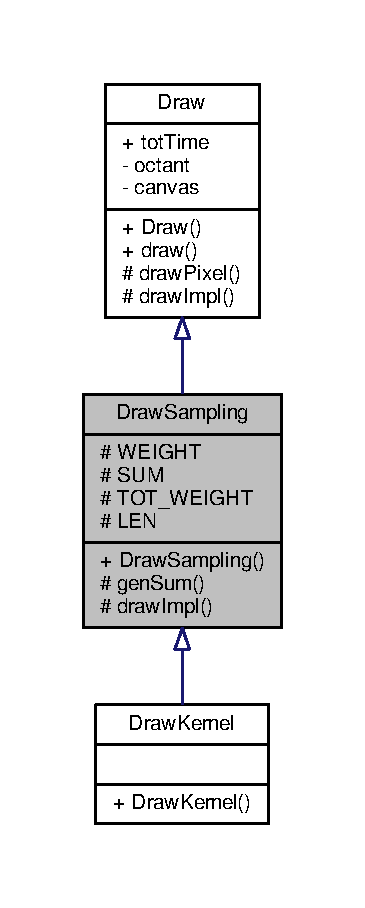
\includegraphics[width=175pt]{classDrawSampling__inherit__graph}
\end{center}
\end{figure}


Collaboration diagram for Draw\+Sampling\+:
\nopagebreak
\begin{figure}[H]
\begin{center}
\leavevmode
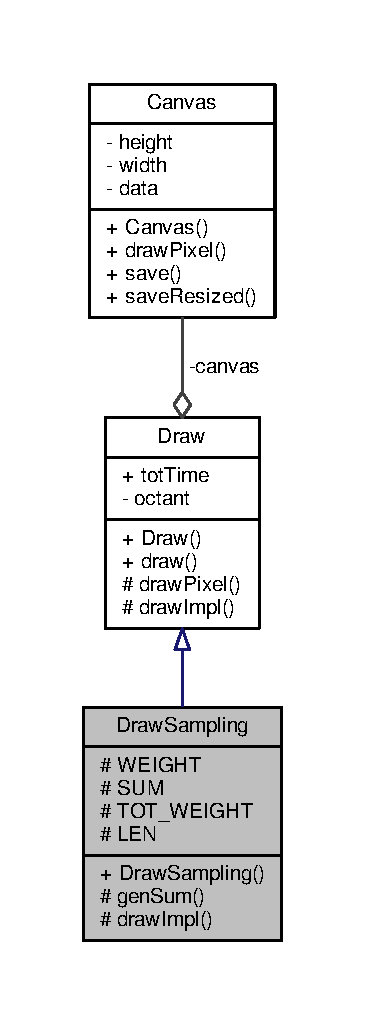
\includegraphics[width=175pt]{classDrawSampling__coll__graph}
\end{center}
\end{figure}
\subsection*{Public Member Functions}
\begin{DoxyCompactItemize}
\item 
\hyperlink{classDrawSampling_aa02ae6778de2385b7451f62f1e03cb1e}{Draw\+Sampling} (\hyperlink{classCanvas}{Canvas} \&\hyperlink{classDraw_a72ed77716d9eb7068414f0e4e00753bd}{canvas})
\end{DoxyCompactItemize}
\subsection*{Protected Types}
\begin{DoxyCompactItemize}
\item 
typedef std\+::array$<$ std\+::array$<$ int, \hyperlink{classDrawSampling_a65a0b2e1d234d93049c4807d32fd009d}{L\+EN} $>$, \hyperlink{classDrawSampling_a65a0b2e1d234d93049c4807d32fd009d}{L\+EN} $>$ \hyperlink{classDrawSampling_a73c5d308c9d35c89746810be84e6834d}{Weight\+Mat}
\begin{DoxyCompactList}\small\item\em Slide length of the fine division. \end{DoxyCompactList}\end{DoxyCompactItemize}
\subsection*{Protected Member Functions}
\begin{DoxyCompactItemize}
\item 
\hyperlink{classDrawSampling_a73c5d308c9d35c89746810be84e6834d}{Weight\+Mat} \hyperlink{classDrawSampling_ac5f43bc9f50a57bb7226f6e971c0fd53}{gen\+Sum} () const 
\item 
void \hyperlink{classDrawSampling_a3d67fd8278cf17d4cb35958aa1a21e31}{draw\+Impl} (int x0, int y0, int x1, int y1, const \hyperlink{canvas_8h_a084a39206618848fb8bc9187d3758c87}{Color} \&color) override
\begin{DoxyCompactList}\small\item\em Implementation. \end{DoxyCompactList}\end{DoxyCompactItemize}
\subsection*{Protected Attributes}
\begin{DoxyCompactItemize}
\item 
\hyperlink{classDrawSampling_a73c5d308c9d35c89746810be84e6834d}{Weight\+Mat} \hyperlink{classDrawSampling_ac76ed88fbade57d7d259fa6bb4ddb312}{W\+E\+I\+G\+HT}
\item 
\hyperlink{classDrawSampling_a73c5d308c9d35c89746810be84e6834d}{Weight\+Mat} \hyperlink{classDrawSampling_a63072a47a8eb23f487f94418c9a27208}{S\+UM}
\item 
int \hyperlink{classDrawSampling_a8ce16ba19af34ba89f7722b7d993143c}{T\+O\+T\+\_\+\+W\+E\+I\+G\+HT}
\end{DoxyCompactItemize}
\subsection*{Static Protected Attributes}
\begin{DoxyCompactItemize}
\item 
static const int \hyperlink{classDrawSampling_a65a0b2e1d234d93049c4807d32fd009d}{L\+EN} = 7
\end{DoxyCompactItemize}
\subsection*{Additional Inherited Members}


\subsection{Detailed Description}
Uniform sampling algorithm. 

\subsection{Member Typedef Documentation}
\index{Draw\+Sampling@{Draw\+Sampling}!Weight\+Mat@{Weight\+Mat}}
\index{Weight\+Mat@{Weight\+Mat}!Draw\+Sampling@{Draw\+Sampling}}
\subsubsection[{\texorpdfstring{Weight\+Mat}{WeightMat}}]{\setlength{\rightskip}{0pt plus 5cm}typedef std\+::array$<$std\+::array$<$int, {\bf L\+EN}$>$, {\bf L\+EN}$>$ {\bf Draw\+Sampling\+::\+Weight\+Mat}\hspace{0.3cm}{\ttfamily [protected]}}\hypertarget{classDrawSampling_a73c5d308c9d35c89746810be84e6834d}{}\label{classDrawSampling_a73c5d308c9d35c89746810be84e6834d}


Slide length of the fine division. 



\subsection{Constructor \& Destructor Documentation}
\index{Draw\+Sampling@{Draw\+Sampling}!Draw\+Sampling@{Draw\+Sampling}}
\index{Draw\+Sampling@{Draw\+Sampling}!Draw\+Sampling@{Draw\+Sampling}}
\subsubsection[{\texorpdfstring{Draw\+Sampling(\+Canvas \&canvas)}{DrawSampling(Canvas &canvas)}}]{\setlength{\rightskip}{0pt plus 5cm}Draw\+Sampling\+::\+Draw\+Sampling (
\begin{DoxyParamCaption}
\item[{{\bf Canvas} \&}]{canvas}
\end{DoxyParamCaption}
)\hspace{0.3cm}{\ttfamily [inline]}}\hypertarget{classDrawSampling_aa02ae6778de2385b7451f62f1e03cb1e}{}\label{classDrawSampling_aa02ae6778de2385b7451f62f1e03cb1e}


\subsection{Member Function Documentation}
\index{Draw\+Sampling@{Draw\+Sampling}!draw\+Impl@{draw\+Impl}}
\index{draw\+Impl@{draw\+Impl}!Draw\+Sampling@{Draw\+Sampling}}
\subsubsection[{\texorpdfstring{draw\+Impl(int x0, int y0, int x1, int y1, const Color \&color) override}{drawImpl(int x0, int y0, int x1, int y1, const Color &color) override}}]{\setlength{\rightskip}{0pt plus 5cm}void Draw\+Sampling\+::draw\+Impl (
\begin{DoxyParamCaption}
\item[{int}]{x0, }
\item[{int}]{y0, }
\item[{int}]{x1, }
\item[{int}]{y1, }
\item[{const {\bf Color} \&}]{color}
\end{DoxyParamCaption}
)\hspace{0.3cm}{\ttfamily [override]}, {\ttfamily [protected]}, {\ttfamily [virtual]}}\hypertarget{classDrawSampling_a3d67fd8278cf17d4cb35958aa1a21e31}{}\label{classDrawSampling_a3d67fd8278cf17d4cb35958aa1a21e31}


Implementation. 

Suppose 0 $<$= slope $<$= 1 

Reimplemented from \hyperlink{classDraw_ac9f2fe7c73db00834df73437767fa3ce}{Draw}.

\index{Draw\+Sampling@{Draw\+Sampling}!gen\+Sum@{gen\+Sum}}
\index{gen\+Sum@{gen\+Sum}!Draw\+Sampling@{Draw\+Sampling}}
\subsubsection[{\texorpdfstring{gen\+Sum() const }{genSum() const }}]{\setlength{\rightskip}{0pt plus 5cm}{\bf Draw\+Sampling\+::\+Weight\+Mat} Draw\+Sampling\+::gen\+Sum (
\begin{DoxyParamCaption}
{}
\end{DoxyParamCaption}
) const\hspace{0.3cm}{\ttfamily [protected]}}\hypertarget{classDrawSampling_ac5f43bc9f50a57bb7226f6e971c0fd53}{}\label{classDrawSampling_ac5f43bc9f50a57bb7226f6e971c0fd53}


\subsection{Member Data Documentation}
\index{Draw\+Sampling@{Draw\+Sampling}!L\+EN@{L\+EN}}
\index{L\+EN@{L\+EN}!Draw\+Sampling@{Draw\+Sampling}}
\subsubsection[{\texorpdfstring{L\+EN}{LEN}}]{\setlength{\rightskip}{0pt plus 5cm}const int Draw\+Sampling\+::\+L\+EN = 7\hspace{0.3cm}{\ttfamily [static]}, {\ttfamily [protected]}}\hypertarget{classDrawSampling_a65a0b2e1d234d93049c4807d32fd009d}{}\label{classDrawSampling_a65a0b2e1d234d93049c4807d32fd009d}
\index{Draw\+Sampling@{Draw\+Sampling}!S\+UM@{S\+UM}}
\index{S\+UM@{S\+UM}!Draw\+Sampling@{Draw\+Sampling}}
\subsubsection[{\texorpdfstring{S\+UM}{SUM}}]{\setlength{\rightskip}{0pt plus 5cm}{\bf Weight\+Mat} Draw\+Sampling\+::\+S\+UM\hspace{0.3cm}{\ttfamily [protected]}}\hypertarget{classDrawSampling_a63072a47a8eb23f487f94418c9a27208}{}\label{classDrawSampling_a63072a47a8eb23f487f94418c9a27208}
\index{Draw\+Sampling@{Draw\+Sampling}!T\+O\+T\+\_\+\+W\+E\+I\+G\+HT@{T\+O\+T\+\_\+\+W\+E\+I\+G\+HT}}
\index{T\+O\+T\+\_\+\+W\+E\+I\+G\+HT@{T\+O\+T\+\_\+\+W\+E\+I\+G\+HT}!Draw\+Sampling@{Draw\+Sampling}}
\subsubsection[{\texorpdfstring{T\+O\+T\+\_\+\+W\+E\+I\+G\+HT}{TOT_WEIGHT}}]{\setlength{\rightskip}{0pt plus 5cm}int Draw\+Sampling\+::\+T\+O\+T\+\_\+\+W\+E\+I\+G\+HT\hspace{0.3cm}{\ttfamily [protected]}}\hypertarget{classDrawSampling_a8ce16ba19af34ba89f7722b7d993143c}{}\label{classDrawSampling_a8ce16ba19af34ba89f7722b7d993143c}
\index{Draw\+Sampling@{Draw\+Sampling}!W\+E\+I\+G\+HT@{W\+E\+I\+G\+HT}}
\index{W\+E\+I\+G\+HT@{W\+E\+I\+G\+HT}!Draw\+Sampling@{Draw\+Sampling}}
\subsubsection[{\texorpdfstring{W\+E\+I\+G\+HT}{WEIGHT}}]{\setlength{\rightskip}{0pt plus 5cm}{\bf Weight\+Mat} Draw\+Sampling\+::\+W\+E\+I\+G\+HT\hspace{0.3cm}{\ttfamily [protected]}}\hypertarget{classDrawSampling_ac76ed88fbade57d7d259fa6bb4ddb312}{}\label{classDrawSampling_ac76ed88fbade57d7d259fa6bb4ddb312}


The documentation for this class was generated from the following files\+:\begin{DoxyCompactItemize}
\item 
\hyperlink{drawsampling_8h}{drawsampling.\+h}\item 
\hyperlink{drawsampling_8cpp}{drawsampling.\+cpp}\end{DoxyCompactItemize}

\hypertarget{classDrawWidth}{}\section{Draw\+Width Class Reference}
\label{classDrawWidth}\index{Draw\+Width@{Draw\+Width}}


\hyperlink{classDraw}{Draw} lines with a width.  




{\ttfamily \#include $<$drawwidth.\+h$>$}



Inheritance diagram for Draw\+Width\+:
\nopagebreak
\begin{figure}[H]
\begin{center}
\leavevmode
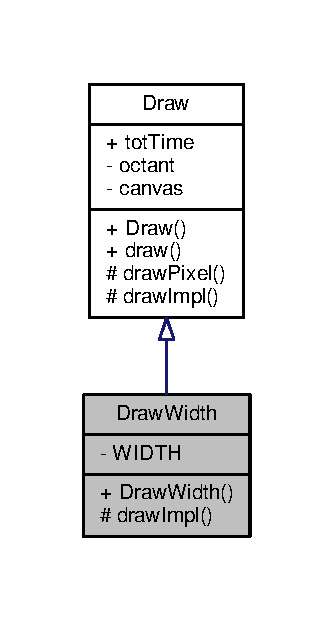
\includegraphics[width=160pt]{classDrawWidth__inherit__graph}
\end{center}
\end{figure}


Collaboration diagram for Draw\+Width\+:
\nopagebreak
\begin{figure}[H]
\begin{center}
\leavevmode
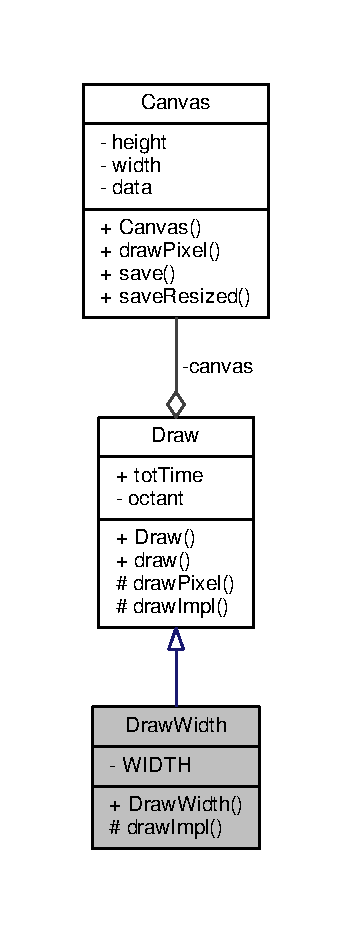
\includegraphics[width=169pt]{classDrawWidth__coll__graph}
\end{center}
\end{figure}
\subsection*{Public Member Functions}
\begin{DoxyCompactItemize}
\item 
\hyperlink{classDrawWidth_af073f8b445c1411582a6f2c2027ec8bd}{Draw\+Width} (\hyperlink{classCanvas}{Canvas} \&\hyperlink{classDraw_a72ed77716d9eb7068414f0e4e00753bd}{canvas}, int \+\_\+width)
\end{DoxyCompactItemize}
\subsection*{Protected Member Functions}
\begin{DoxyCompactItemize}
\item 
void \hyperlink{classDrawWidth_a566f96378bc924c2362551c062612131}{draw\+Impl} (int x0, int y0, int x1, int y1, const \hyperlink{canvas_8h_a084a39206618848fb8bc9187d3758c87}{Color} \&color) override
\begin{DoxyCompactList}\small\item\em Implementation. \end{DoxyCompactList}\end{DoxyCompactItemize}
\subsection*{Private Attributes}
\begin{DoxyCompactItemize}
\item 
const int \hyperlink{classDrawWidth_a4cad2704fa9da370c78651d704fb1d96}{W\+I\+D\+TH}
\end{DoxyCompactItemize}
\subsection*{Additional Inherited Members}


\subsection{Detailed Description}
\hyperlink{classDraw}{Draw} lines with a width. 

\subsection{Constructor \& Destructor Documentation}
\index{Draw\+Width@{Draw\+Width}!Draw\+Width@{Draw\+Width}}
\index{Draw\+Width@{Draw\+Width}!Draw\+Width@{Draw\+Width}}
\subsubsection[{\texorpdfstring{Draw\+Width(\+Canvas \&canvas, int \+\_\+width)}{DrawWidth(Canvas &canvas, int _width)}}]{\setlength{\rightskip}{0pt plus 5cm}Draw\+Width\+::\+Draw\+Width (
\begin{DoxyParamCaption}
\item[{{\bf Canvas} \&}]{canvas, }
\item[{int}]{\+\_\+width}
\end{DoxyParamCaption}
)\hspace{0.3cm}{\ttfamily [inline]}}\hypertarget{classDrawWidth_af073f8b445c1411582a6f2c2027ec8bd}{}\label{classDrawWidth_af073f8b445c1411582a6f2c2027ec8bd}


\subsection{Member Function Documentation}
\index{Draw\+Width@{Draw\+Width}!draw\+Impl@{draw\+Impl}}
\index{draw\+Impl@{draw\+Impl}!Draw\+Width@{Draw\+Width}}
\subsubsection[{\texorpdfstring{draw\+Impl(int x0, int y0, int x1, int y1, const Color \&color) override}{drawImpl(int x0, int y0, int x1, int y1, const Color &color) override}}]{\setlength{\rightskip}{0pt plus 5cm}void Draw\+Width\+::draw\+Impl (
\begin{DoxyParamCaption}
\item[{int}]{x0, }
\item[{int}]{y0, }
\item[{int}]{x1, }
\item[{int}]{y1, }
\item[{const {\bf Color} \&}]{color}
\end{DoxyParamCaption}
)\hspace{0.3cm}{\ttfamily [override]}, {\ttfamily [protected]}, {\ttfamily [virtual]}}\hypertarget{classDrawWidth_a566f96378bc924c2362551c062612131}{}\label{classDrawWidth_a566f96378bc924c2362551c062612131}


Implementation. 

Suppose 0 $<$= slope $<$= 1 

Reimplemented from \hyperlink{classDraw_ac9f2fe7c73db00834df73437767fa3ce}{Draw}.



\subsection{Member Data Documentation}
\index{Draw\+Width@{Draw\+Width}!W\+I\+D\+TH@{W\+I\+D\+TH}}
\index{W\+I\+D\+TH@{W\+I\+D\+TH}!Draw\+Width@{Draw\+Width}}
\subsubsection[{\texorpdfstring{W\+I\+D\+TH}{WIDTH}}]{\setlength{\rightskip}{0pt plus 5cm}const int Draw\+Width\+::\+W\+I\+D\+TH\hspace{0.3cm}{\ttfamily [private]}}\hypertarget{classDrawWidth_a4cad2704fa9da370c78651d704fb1d96}{}\label{classDrawWidth_a4cad2704fa9da370c78651d704fb1d96}


The documentation for this class was generated from the following files\+:\begin{DoxyCompactItemize}
\item 
\hyperlink{drawwidth_8h}{drawwidth.\+h}\item 
\hyperlink{drawwidth_8cpp}{drawwidth.\+cpp}\end{DoxyCompactItemize}

\chapter{File Documentation}
\hypertarget{canvas_8h}{}\section{canvas.\+h File Reference}
\label{canvas_8h}\index{canvas.\+h@{canvas.\+h}}
{\ttfamily \#include $<$iostream$>$}\\*
{\ttfamily \#include $<$opencv2/opencv.\+hpp$>$}\\*
Include dependency graph for canvas.\+h\+:
\nopagebreak
\begin{figure}[H]
\begin{center}
\leavevmode
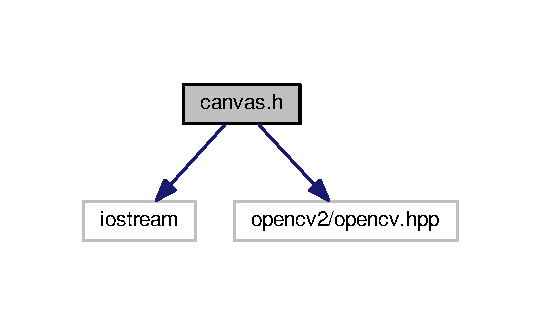
\includegraphics[width=260pt]{canvas_8h__incl}
\end{center}
\end{figure}
This graph shows which files directly or indirectly include this file\+:
\nopagebreak
\begin{figure}[H]
\begin{center}
\leavevmode
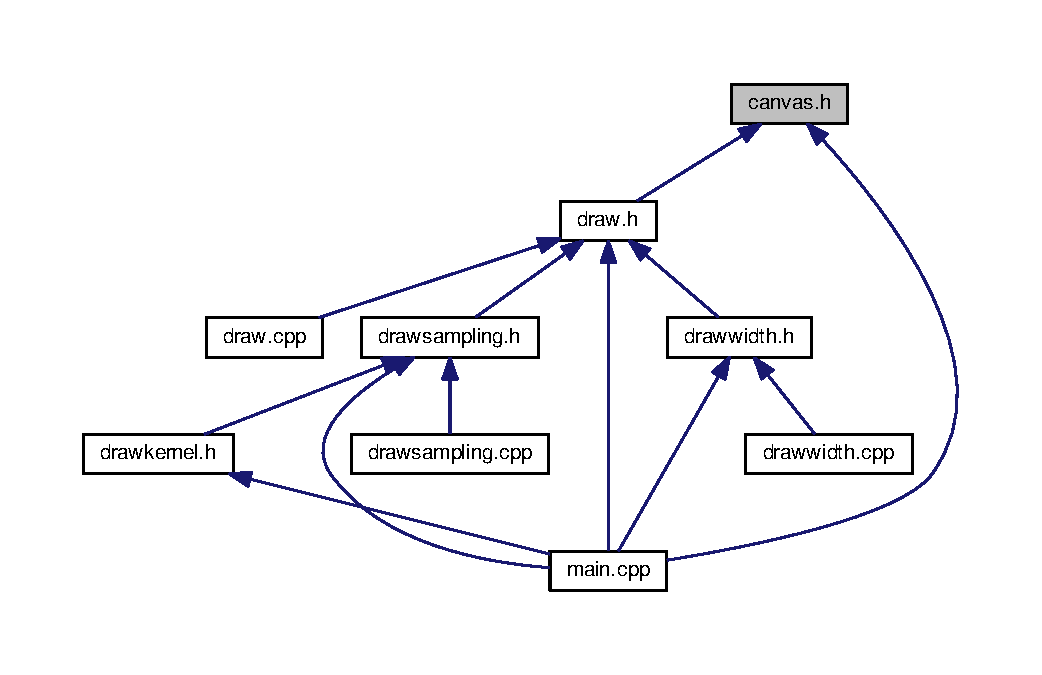
\includegraphics[width=350pt]{canvas_8h__dep__incl}
\end{center}
\end{figure}
\subsection*{Classes}
\begin{DoxyCompactItemize}
\item 
class \hyperlink{classCanvas}{Canvas}
\begin{DoxyCompactList}\small\item\em Interface to Open\+CV. \end{DoxyCompactList}\end{DoxyCompactItemize}
\subsection*{Typedefs}
\begin{DoxyCompactItemize}
\item 
typedef cv\+::\+Vec3b \hyperlink{canvas_8h_a084a39206618848fb8bc9187d3758c87}{Color}
\end{DoxyCompactItemize}


\subsection{Typedef Documentation}
\index{canvas.\+h@{canvas.\+h}!Color@{Color}}
\index{Color@{Color}!canvas.\+h@{canvas.\+h}}
\subsubsection[{\texorpdfstring{Color}{Color}}]{\setlength{\rightskip}{0pt plus 5cm}typedef cv\+::\+Vec3b {\bf Color}}\hypertarget{canvas_8h_a084a39206618848fb8bc9187d3758c87}{}\label{canvas_8h_a084a39206618848fb8bc9187d3758c87}

\hypertarget{const_8h}{}\section{const.\+h File Reference}
\label{const_8h}\index{const.\+h@{const.\+h}}
{\ttfamily \#include $<$cmath$>$}\\*
Include dependency graph for const.\+h\+:
\nopagebreak
\begin{figure}[H]
\begin{center}
\leavevmode
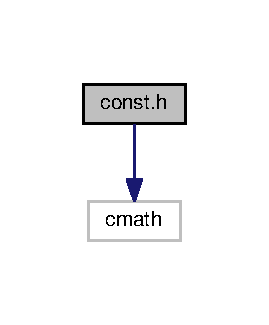
\includegraphics[width=129pt]{const_8h__incl}
\end{center}
\end{figure}
This graph shows which files directly or indirectly include this file\+:
\nopagebreak
\begin{figure}[H]
\begin{center}
\leavevmode
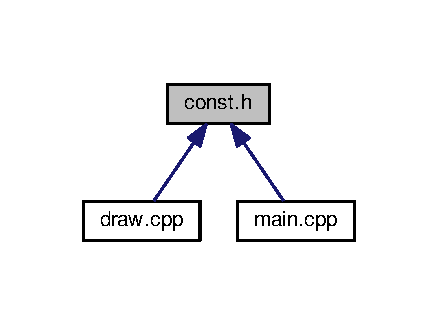
\includegraphics[width=210pt]{const_8h__dep__incl}
\end{center}
\end{figure}
\subsection*{Variables}
\begin{DoxyCompactItemize}
\item 
const int \hyperlink{const_8h_a3b7a268600e76f03faa44ba7cab3eeff}{I\+M\+G\+\_\+\+H\+E\+I\+G\+HT} = 400
\item 
const int \hyperlink{const_8h_a9757ae46d7ae705a16b7b2a51472b764}{I\+M\+G\+\_\+\+W\+I\+D\+TH} = 400
\item 
const int \hyperlink{const_8h_adc2de338d3d280c2ef8805f7e21c63fc}{L\+I\+N\+E\+\_\+\+C\+NT} = 36
\item 
const double \hyperlink{const_8h_a43016d873124d39034edb8cd164794db}{pi} = acos(-\/1)
\end{DoxyCompactItemize}


\subsection{Variable Documentation}
\index{const.\+h@{const.\+h}!I\+M\+G\+\_\+\+H\+E\+I\+G\+HT@{I\+M\+G\+\_\+\+H\+E\+I\+G\+HT}}
\index{I\+M\+G\+\_\+\+H\+E\+I\+G\+HT@{I\+M\+G\+\_\+\+H\+E\+I\+G\+HT}!const.\+h@{const.\+h}}
\subsubsection[{\texorpdfstring{I\+M\+G\+\_\+\+H\+E\+I\+G\+HT}{IMG_HEIGHT}}]{\setlength{\rightskip}{0pt plus 5cm}const int I\+M\+G\+\_\+\+H\+E\+I\+G\+HT = 400}\hypertarget{const_8h_a3b7a268600e76f03faa44ba7cab3eeff}{}\label{const_8h_a3b7a268600e76f03faa44ba7cab3eeff}
\index{const.\+h@{const.\+h}!I\+M\+G\+\_\+\+W\+I\+D\+TH@{I\+M\+G\+\_\+\+W\+I\+D\+TH}}
\index{I\+M\+G\+\_\+\+W\+I\+D\+TH@{I\+M\+G\+\_\+\+W\+I\+D\+TH}!const.\+h@{const.\+h}}
\subsubsection[{\texorpdfstring{I\+M\+G\+\_\+\+W\+I\+D\+TH}{IMG_WIDTH}}]{\setlength{\rightskip}{0pt plus 5cm}const int I\+M\+G\+\_\+\+W\+I\+D\+TH = 400}\hypertarget{const_8h_a9757ae46d7ae705a16b7b2a51472b764}{}\label{const_8h_a9757ae46d7ae705a16b7b2a51472b764}
\index{const.\+h@{const.\+h}!L\+I\+N\+E\+\_\+\+C\+NT@{L\+I\+N\+E\+\_\+\+C\+NT}}
\index{L\+I\+N\+E\+\_\+\+C\+NT@{L\+I\+N\+E\+\_\+\+C\+NT}!const.\+h@{const.\+h}}
\subsubsection[{\texorpdfstring{L\+I\+N\+E\+\_\+\+C\+NT}{LINE_CNT}}]{\setlength{\rightskip}{0pt plus 5cm}const int L\+I\+N\+E\+\_\+\+C\+NT = 36}\hypertarget{const_8h_adc2de338d3d280c2ef8805f7e21c63fc}{}\label{const_8h_adc2de338d3d280c2ef8805f7e21c63fc}
\index{const.\+h@{const.\+h}!pi@{pi}}
\index{pi@{pi}!const.\+h@{const.\+h}}
\subsubsection[{\texorpdfstring{pi}{pi}}]{\setlength{\rightskip}{0pt plus 5cm}const double pi = acos(-\/1)}\hypertarget{const_8h_a43016d873124d39034edb8cd164794db}{}\label{const_8h_a43016d873124d39034edb8cd164794db}

\hypertarget{draw_8cpp}{}\section{draw.\+cpp File Reference}
\label{draw_8cpp}\index{draw.\+cpp@{draw.\+cpp}}
{\ttfamily \#include $<$cassert$>$}\\*
{\ttfamily \#include $<$algorithm$>$}\\*
{\ttfamily \#include \char`\"{}draw.\+h\char`\"{}}\\*
{\ttfamily \#include \char`\"{}const.\+h\char`\"{}}\\*
Include dependency graph for draw.\+cpp\+:\nopagebreak
\begin{figure}[H]
\begin{center}
\leavevmode
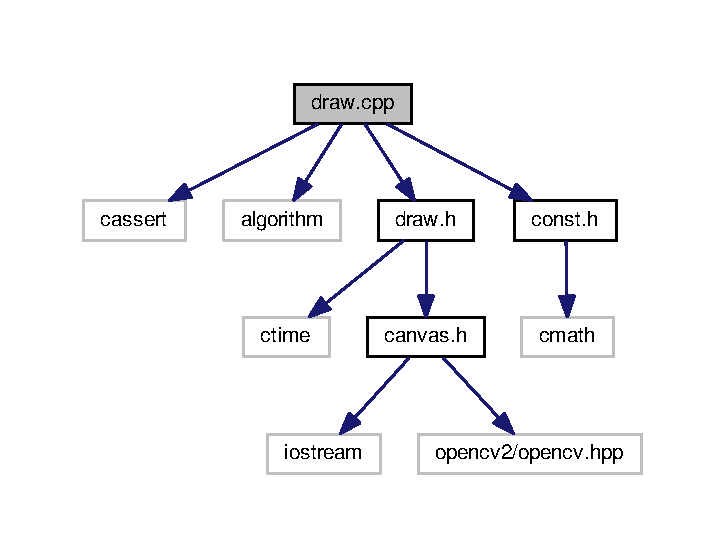
\includegraphics[width=348pt]{draw_8cpp__incl}
\end{center}
\end{figure}

\hypertarget{draw_8h}{}\section{draw.\+h File Reference}
\label{draw_8h}\index{draw.\+h@{draw.\+h}}
{\ttfamily \#include $<$ctime$>$}\\*
{\ttfamily \#include \char`\"{}canvas.\+h\char`\"{}}\\*
Include dependency graph for draw.\+h\+:\nopagebreak
\begin{figure}[H]
\begin{center}
\leavevmode
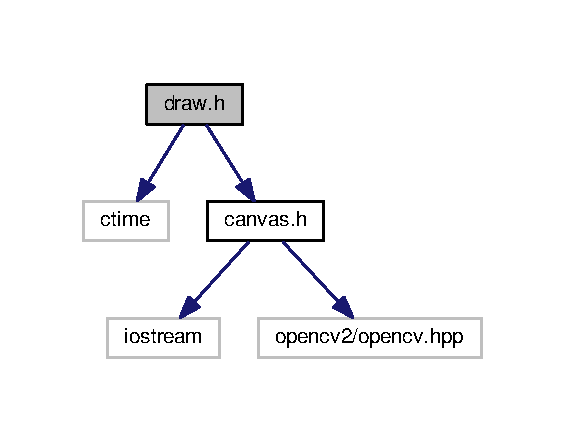
\includegraphics[width=271pt]{draw_8h__incl}
\end{center}
\end{figure}
This graph shows which files directly or indirectly include this file\+:\nopagebreak
\begin{figure}[H]
\begin{center}
\leavevmode
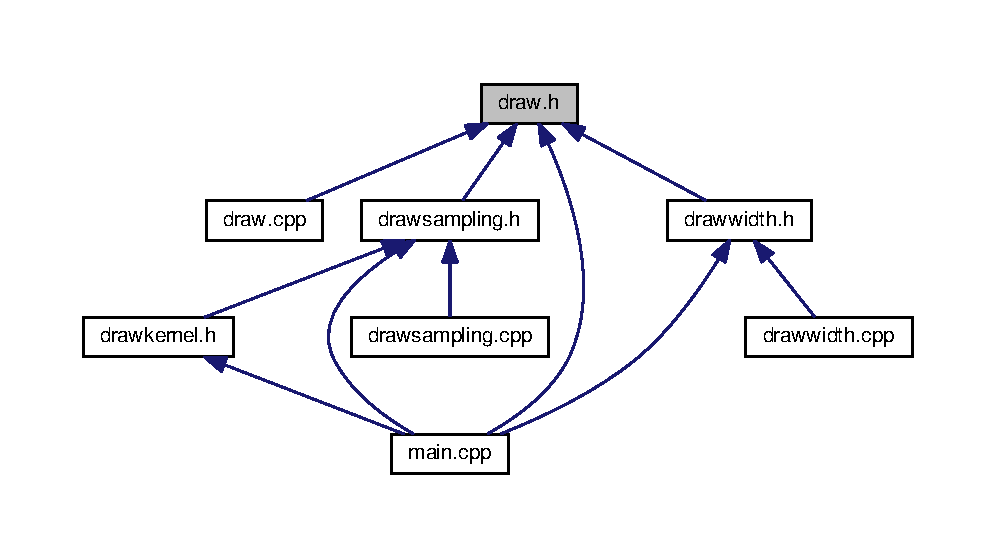
\includegraphics[width=350pt]{draw_8h__dep__incl}
\end{center}
\end{figure}
\subsection*{Classes}
\begin{DoxyCompactItemize}
\item 
class \hyperlink{classDraw}{Draw}
\begin{DoxyCompactList}\small\item\em Plain draw-\/line algorithm. \end{DoxyCompactList}\end{DoxyCompactItemize}

\hypertarget{drawkernel_8h}{}\section{drawkernel.\+h File Reference}
\label{drawkernel_8h}\index{drawkernel.\+h@{drawkernel.\+h}}
{\ttfamily \#include $<$iostream$>$}\\*
{\ttfamily \#include \char`\"{}drawsampling.\+h\char`\"{}}\\*
Include dependency graph for drawkernel.\+h\+:\nopagebreak
\begin{figure}[H]
\begin{center}
\leavevmode
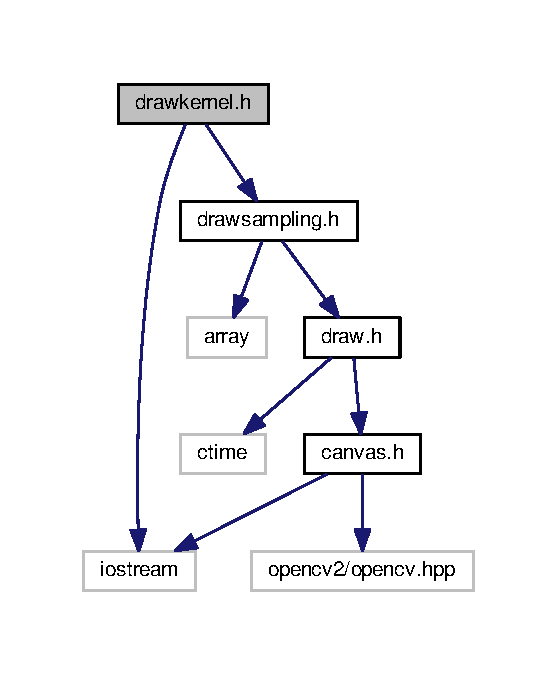
\includegraphics[width=268pt]{drawkernel_8h__incl}
\end{center}
\end{figure}
This graph shows which files directly or indirectly include this file\+:\nopagebreak
\begin{figure}[H]
\begin{center}
\leavevmode
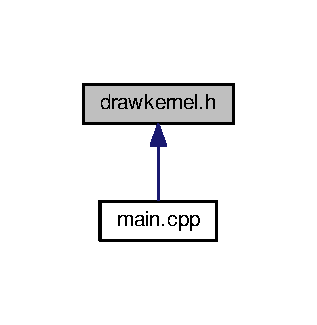
\includegraphics[width=152pt]{drawkernel_8h__dep__incl}
\end{center}
\end{figure}
\subsection*{Classes}
\begin{DoxyCompactItemize}
\item 
class \hyperlink{classDrawKernel}{Draw\+Kernel}
\begin{DoxyCompactList}\small\item\em Kernel algorithm, i.\+e. \end{DoxyCompactList}\end{DoxyCompactItemize}

\hypertarget{drawsampling_8cpp}{}\section{drawsampling.\+cpp File Reference}
\label{drawsampling_8cpp}\index{drawsampling.\+cpp@{drawsampling.\+cpp}}
{\ttfamily \#include $<$cstdlib$>$}\\*
{\ttfamily \#include \char`\"{}drawsampling.\+h\char`\"{}}\\*
Include dependency graph for drawsampling.\+cpp\+:
\nopagebreak
\begin{figure}[H]
\begin{center}
\leavevmode
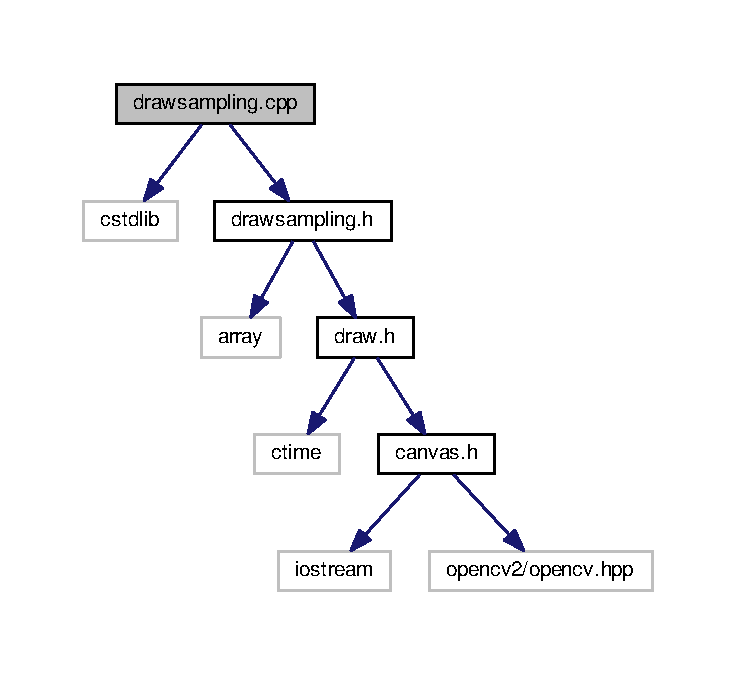
\includegraphics[width=350pt]{drawsampling_8cpp__incl}
\end{center}
\end{figure}

\hypertarget{drawsampling_8h}{}\section{drawsampling.\+h File Reference}
\label{drawsampling_8h}\index{drawsampling.\+h@{drawsampling.\+h}}
{\ttfamily \#include $<$array$>$}\\*
{\ttfamily \#include \char`\"{}draw.\+h\char`\"{}}\\*
Include dependency graph for drawsampling.\+h\+:
\nopagebreak
\begin{figure}[H]
\begin{center}
\leavevmode
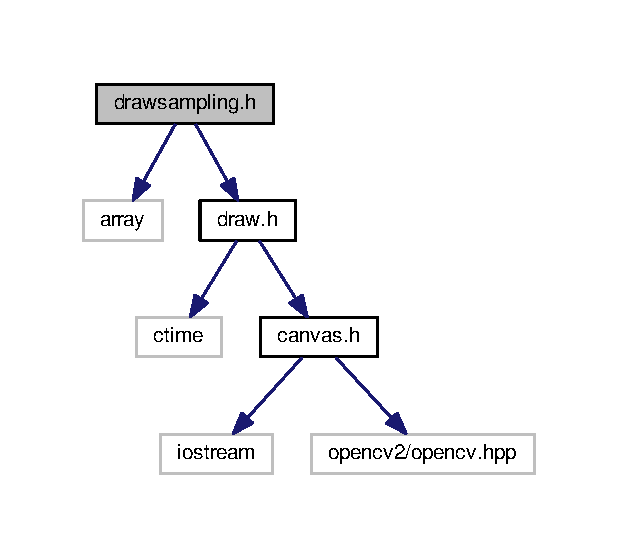
\includegraphics[width=297pt]{drawsampling_8h__incl}
\end{center}
\end{figure}
This graph shows which files directly or indirectly include this file\+:
\nopagebreak
\begin{figure}[H]
\begin{center}
\leavevmode
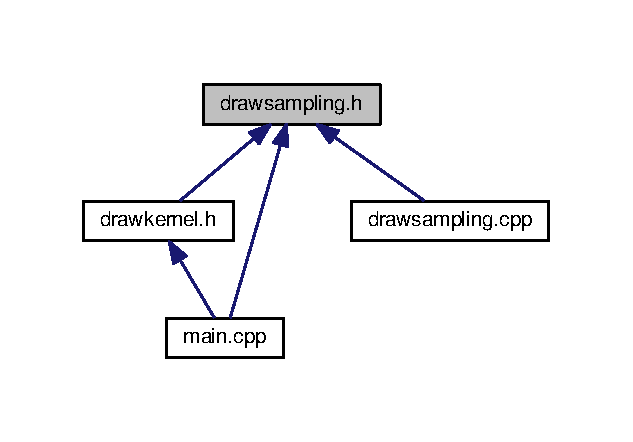
\includegraphics[width=304pt]{drawsampling_8h__dep__incl}
\end{center}
\end{figure}
\subsection*{Classes}
\begin{DoxyCompactItemize}
\item 
class \hyperlink{classDrawSampling}{Draw\+Sampling}
\begin{DoxyCompactList}\small\item\em Uniform sampling algorithm. \end{DoxyCompactList}\end{DoxyCompactItemize}

\hypertarget{drawwidth_8cpp}{}\section{drawwidth.\+cpp File Reference}
\label{drawwidth_8cpp}\index{drawwidth.\+cpp@{drawwidth.\+cpp}}
{\ttfamily \#include \char`\"{}drawwidth.\+h\char`\"{}}\\*
Include dependency graph for drawwidth.\+cpp\+:
\nopagebreak
\begin{figure}[H]
\begin{center}
\leavevmode
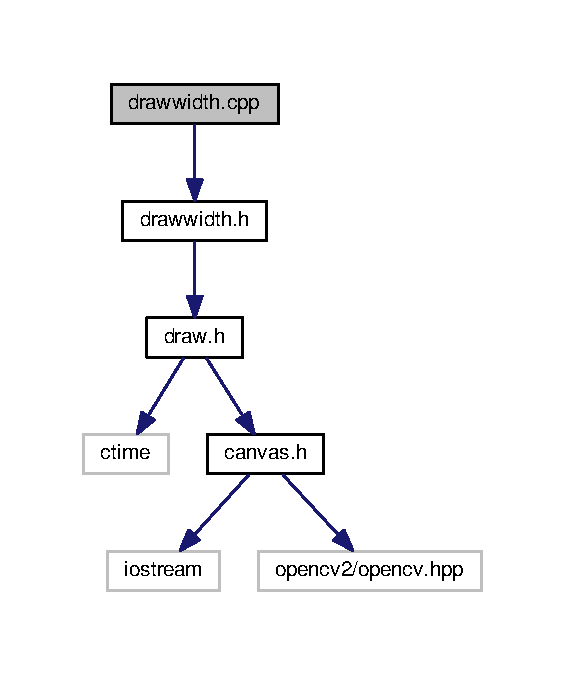
\includegraphics[width=271pt]{drawwidth_8cpp__incl}
\end{center}
\end{figure}

\hypertarget{drawwidth_8h}{}\section{drawwidth.\+h File Reference}
\label{drawwidth_8h}\index{drawwidth.\+h@{drawwidth.\+h}}
{\ttfamily \#include \char`\"{}draw.\+h\char`\"{}}\\*
Include dependency graph for drawwidth.\+h\+:\nopagebreak
\begin{figure}[H]
\begin{center}
\leavevmode
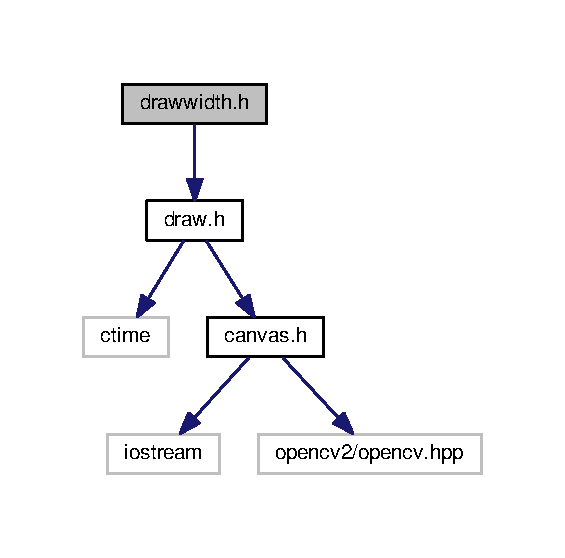
\includegraphics[width=271pt]{drawwidth_8h__incl}
\end{center}
\end{figure}
This graph shows which files directly or indirectly include this file\+:\nopagebreak
\begin{figure}[H]
\begin{center}
\leavevmode
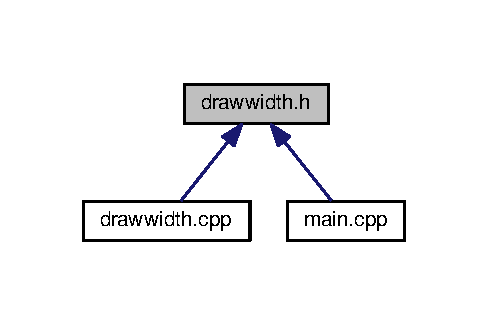
\includegraphics[width=234pt]{drawwidth_8h__dep__incl}
\end{center}
\end{figure}
\subsection*{Classes}
\begin{DoxyCompactItemize}
\item 
class \hyperlink{classDrawWidth}{Draw\+Width}
\begin{DoxyCompactList}\small\item\em \hyperlink{classDraw}{Draw} lines with a width. \end{DoxyCompactList}\end{DoxyCompactItemize}

\hypertarget{main_8cpp}{}\section{main.\+cpp File Reference}
\label{main_8cpp}\index{main.\+cpp@{main.\+cpp}}
{\ttfamily \#include $<$cmath$>$}\\*
{\ttfamily \#include $<$algorithm$>$}\\*
{\ttfamily \#include $<$opencv2/opencv.\+hpp$>$}\\*
{\ttfamily \#include \char`\"{}const.\+h\char`\"{}}\\*
{\ttfamily \#include \char`\"{}canvas.\+h\char`\"{}}\\*
{\ttfamily \#include \char`\"{}draw.\+h\char`\"{}}\\*
{\ttfamily \#include \char`\"{}drawwidth.\+h\char`\"{}}\\*
{\ttfamily \#include \char`\"{}drawkernel.\+h\char`\"{}}\\*
{\ttfamily \#include \char`\"{}drawsampling.\+h\char`\"{}}\\*
Include dependency graph for main.\+cpp\+:\nopagebreak
\begin{figure}[H]
\begin{center}
\leavevmode
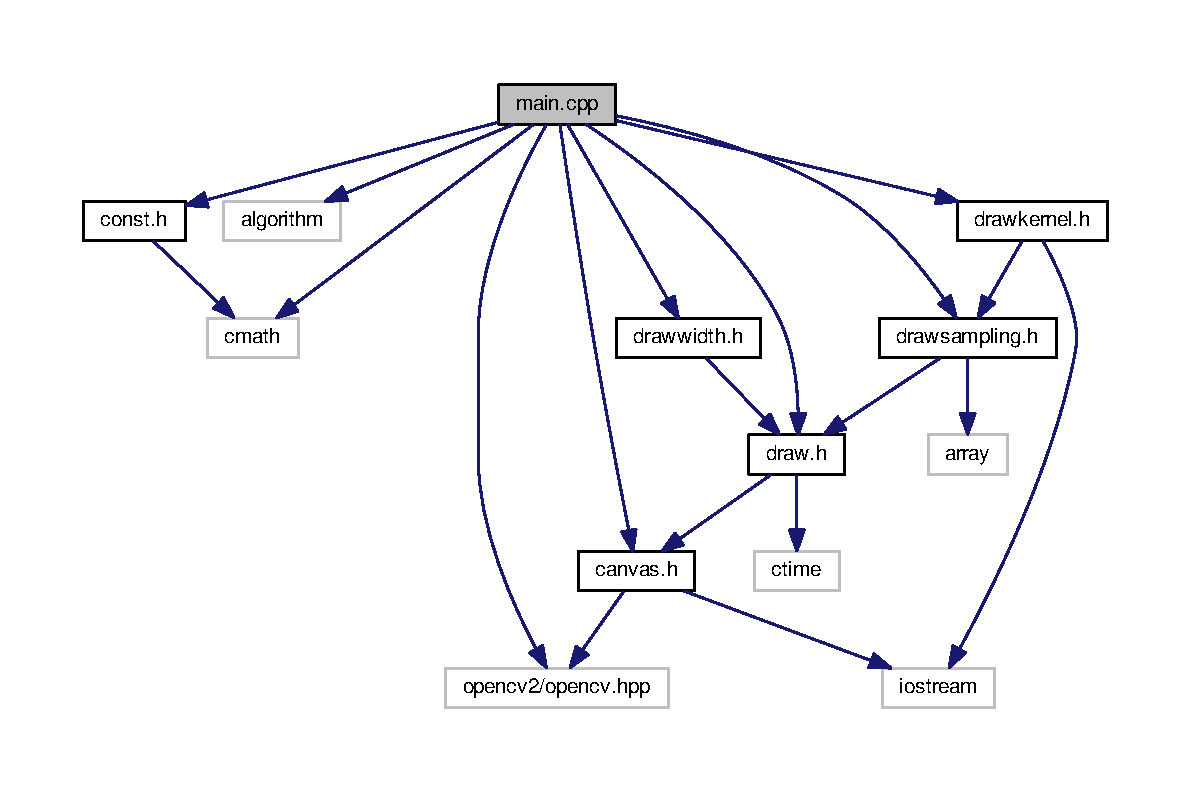
\includegraphics[width=350pt]{main_8cpp__incl}
\end{center}
\end{figure}
\subsection*{Functions}
\begin{DoxyCompactItemize}
\item 
int \hyperlink{main_8cpp_ae66f6b31b5ad750f1fe042a706a4e3d4}{main} ()
\end{DoxyCompactItemize}


\subsection{Function Documentation}
\index{main.\+cpp@{main.\+cpp}!main@{main}}
\index{main@{main}!main.\+cpp@{main.\+cpp}}
\subsubsection[{\texorpdfstring{main()}{main()}}]{\setlength{\rightskip}{0pt plus 5cm}int main (
\begin{DoxyParamCaption}
{}
\end{DoxyParamCaption}
)}\hypertarget{main_8cpp_ae66f6b31b5ad750f1fe042a706a4e3d4}{}\label{main_8cpp_ae66f6b31b5ad750f1fe042a706a4e3d4}

%--- End generated contents ---

% Index
\backmatter
\newpage
\phantomsection
\clearemptydoublepage
\addcontentsline{toc}{chapter}{Index}
\printindex

\end{document}
